\documentclass[12pt]{article}
% For reading variables from external file
\usepackage{caption} 
\usepackage{subcaption} 
\usepackage{datatool}
\usepackage{graphicx}
\usepackage{parskip} 
\usepackage[margin=2cm]{geometry} 
\DTLsetseparator{,}

\begin{document}
% Usage: \dat{variable-name}
%   This prints the value of the variable to the document
\DTLloaddb[noheader, keys={thekey,thevalue}]{dat}{../data/derived/report-summary-data.csv}
\newcommand{\dat}[1]{\DTLfetch{dat}{thekey}{#1}{thevalue}}

\section*{Estimating the magnitude of completion}%
\label{sec:Estimating the magnitude of completion}

Test value of \dat{x1} and \dat{x2}.

We get a $M_c$ estimate of \dat{mc}.



\begin{figure}[htp]
\centering
\begin{subfigure}[b]{0.49\textwidth}
    \centering
    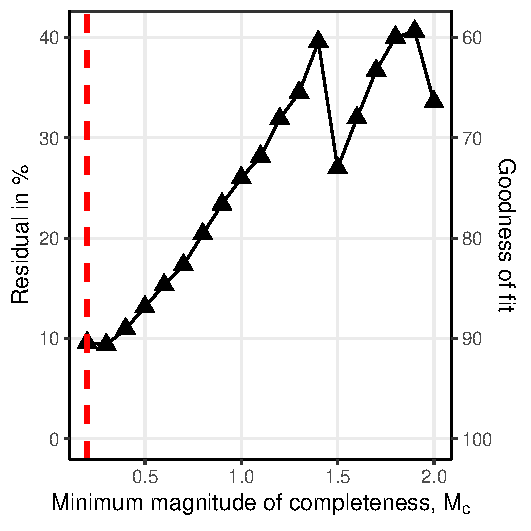
\includegraphics[scale=1.0]{../outputs/figures/goodness-of-fit.pdf}
    \caption{TODO}
    \label{fig:goodness}
\end{subfigure}
\hfill
\begin{subfigure}[b]{0.49\textwidth}
    \centering
    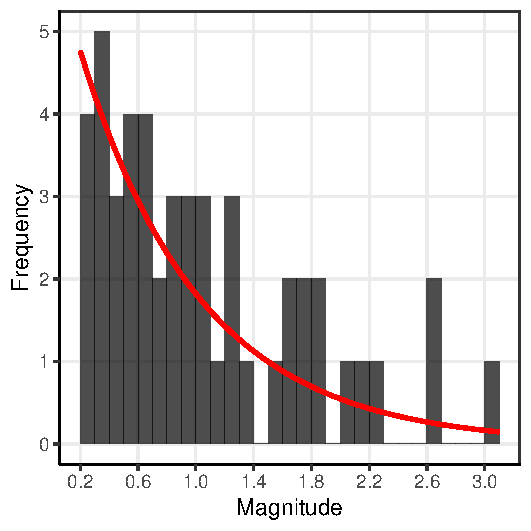
\includegraphics[scale=1.0]{../outputs/figures/earthquake-histogram.pdf}
    \caption{Earthquake frequencies for magnitudes above $M_c=$ TODO}
    \label{fig:hist}
\end{subfigure}
\caption{TODO}
\label{fig:figs1}
\end{figure}



% Estimate Mc using
%
% Minimum Magnitude of Completeness in Earthquake Catalogs:
% Examples from Alaska, the Western United States, and Japan
% by Stefan Wiemer and Max Wyss (see earthquakes in DOwnloads)
%
% https://agupubs.onlinelibrary.wiley.com/doi/full/10.26464/epp2018015?saml_referrer
%
% https://agupubs.onlinelibrary.wiley.com/doi/full/10.26464/epp2018015?saml_referrer
%
% Need to figure out how to perform the estimation again, because don't get working plots...
%
% summary here...
%
% https://pubs.geoscienceworld.org/ssa/bssa/article/90/4/859/120531/Minimum-Magnitude-of-Completeness-in-Earthquake
%
% Use this ^^ ?
%
% Downloads/CORSSA as well...
%
% When get back, just try to make the estimate as simple as possible i.e. just use idea of shifting data by Mc and then using exponential MLE or something and use a different metric to measure goodness of fit, for example binned MSE or something, averaged over number of "predictions" made instead of sum over true values...

\end{document}
